%!TEX root = ../main.tex

\chapter{Clustering}
\label{cha:clustering}

Il clustering è con ogni probabilità il più importante problema di \textbf{apprendimento non supervisionato}: l'obiettivo che si pone è organizzare dati non classificati in gruppi, detti \textbf{cluster}, i cui membri sono simili secondo qualche criterio.

Sebbene non esista una definizione formale universalmente accettata, tutti concordano nell'affermare che un cluster deve soddisfare i seguenti criteri:
\begin{itemize}
	\item \textbf{criterio interno}: tutti gli oggetti all'\emph{interno} di un cluster devono essere il più possibile simili tra loro;
	\item \textbf{criterio esterno}: tutti gli oggetti all'\emph{esterno} di un cluster devono essere il più possibile dissimili rispetto a quelli contenuti al suo interno.
\end{itemize}
A seconda dell'input che viene fornito all'algoritmo, si distingue tra:
\begin{itemize}
	\item clustering \textbf{feature-based} (o \emph{central} clustering), dove gli oggetti sono rappresentati mediante vettori di caratteristiche;
	\item clustering \textbf{pairwise}, dove viene fornita una \textbf{matrice di similarità} tra gli oggetti.
\end{itemize}
Un approccio feature-based in alcuni casi può non essere applicabile, in quanto non si riesce a fornire una rappresentazione vettoriale degli oggetti su cui fare clustering, mentre è possibile determinarne la similarità: un esempio è dato da oggetti che sono rappresentati mediante grafi.

È utile distinguere il classico approccio al clustering dalla sua formulazione più moderna. Nel caso \textbf{classico}, l'obiettivo del clustering è di \textbf{partizionare} gli oggetti in insiemi massimalmente omogenei, il cui numero è tipicamente dato come input all'algoritmo; secondo il nuovo approccio:
\begin{itemize}
	\item il numero di cluster non è necessario, in quanto vengono estratti sequenzialmente;
	\item è possibile non assegnare degli elementi, utile nel caso di segmentazione di immagini o one-class clustering;
	\item è possibile estrarre cluster sovrapposti.
\end{itemize}

\section{K-means}
\label{sec:k_means}

K-means è probabilmente il più famoso algoritmo di clustering feature-based. Dato un insieme di osservazioni $\{\vec{x}_1, \dots, \vec{x}_n\}$, dove $\vec{x}_i$ è un vettore $m$-dimensionale, e il numero desiderato di cluster $K$, lo scopo dell'algoritmo è di trovare un assegnamento di dati ai cluster e vettori $\vec{\mu}_k$ ($k = 1, \dots, K$), che rappresentano i centroidi dei cluster, tali per cui la distanza dei dati dal centroide del gruppo cui sono stati assegnati sia minima.

Sia $\mat{R} = (r_{ij})$ una matrice $n \times K$ tale per cui $r_{ij} = 1$ se $\vec{x}_i$ è assegnato al cluster $j$ e $0$ altrimenti. L'algoritmo minimizza la \textbf{misura di distorsione}
\begin{displaymath}
	J = \sum_i \sum_k r_{ik} \| \vec{x}_i - \vec{\mu}_k \|^2
\end{displaymath}
iterando i seguenti step:
\begin{itemize}
	\item minimizzare $J$ rispetto a $\mat{R}$, tenendo i centroidi fissi:
	\begin{displaymath}
		r_{ij} = \begin{cases}
 			1 & \text{se } j = \argmin_k \|\vec{x}_i - \vec{\mu}_k\|^2 \\
 			0 & \text{altrimenti}
 		\end{cases}
	\end{displaymath}
	\item minimizzare $J$ rispetto $\vec{\mu}_k$, tenendo gli assegnamenti fissi:
	\begin{displaymath}
		\vec{\mu}_k = \frac{\sum_i r_{ik} \vec{x}_i}{\sum_i r_{ik}}
	\end{displaymath}
\end{itemize}
L'algoritmo viene arrestato quando non viene prodotta alcuna variazione negli assegnamenti oppure dopo un numero fisso di iterazioni: trattandosi di un problema NP-difficile, non è dato sapere a priori se l'algoritmo converga o meno.

Per quanto riguarda l'inizializzazione dei centroidi, questi vengono tipicamente scelti in maniera casuale dall'insieme delle osservazioni.

\begin{figure}[h!]
	\centering
	\subfigure{
	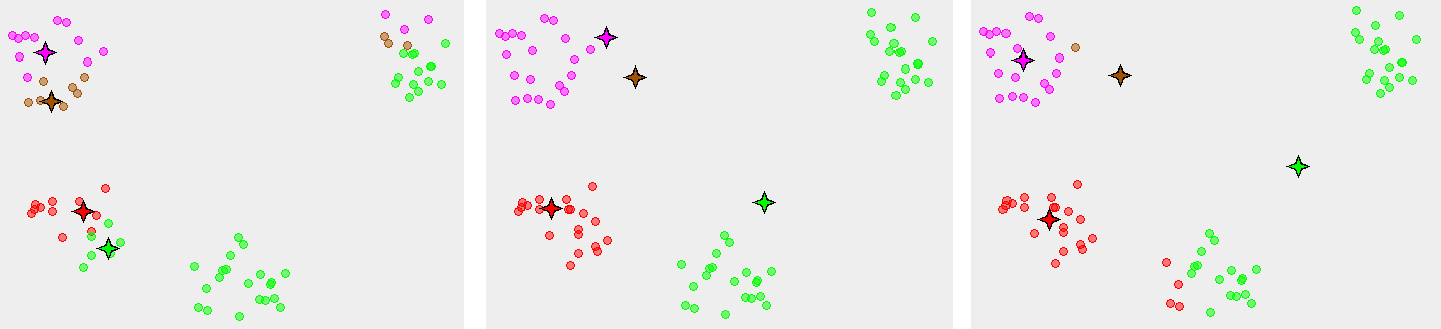
\includegraphics[width=12cm]{images/kmeans}
	}
	\subfigure{
	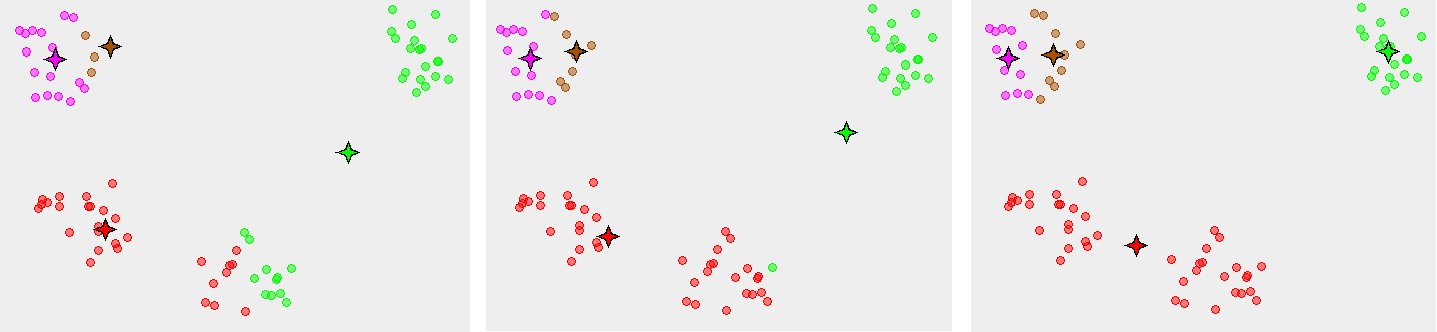
\includegraphics[width=12cm]{images/kmeans2}
	}
	\caption[Convergenza di K-means]{Convergenza (dopo 5 iterazioni) di K-means ad un minimo locale.}
\end{figure}

\section{Normalized Cut}
\label{sec:normalized_cut}

\textbf{Normalized cut} è un algoritmo di clustering pairwise che utilizza tecniche della teoria spettrale dei grafi.

Sia $G = (V, E, w)$ un grafo pesato, dove $V$ è l'insieme degli oggetti su cui fare clustering, $E$ è l'insieme degli archi che indicano le relazioni tra gli oggetti e $w$ è la funzione peso che assegna la similarità a coppie di vertici connessi. L'obiettivo è di individuare un partizionamento non banale $(J, K)$ dei nodi in $V$ tale da minimizzare
\begin{displaymath}
	\textsc{NCut}(J, K) = \frac{\textsc{Cut}(J, K)}{\textsc{Assoc}(J, V)} + \frac{\textsc{Cut}(J, K)}{\textsc{Assoc}(K, V)}
\end{displaymath}
dove:
\begin{align*}
	\textsc{Cut}(J, K) &= \sum_{\substack{u \in J \\ t \in K}} w(u, t) & \textsc{Assoc}(J, V) &= \sum_{\substack{u \in J \\ t \in V}} w(u, t)
\end{align*}
Sia $\vec{y}$ un vettore $|V|$-dimensionale, dove
\begin{displaymath}
	y_i = \begin{cases}
 		1 & \text{se } i \in J \\
 		0 & \text{altrimenti}
 	\end{cases}
\end{displaymath}
$\mat{D} = (d_{ij})$ la matrice diagonale dove $d_{ii} = \sum_j w_{ij}$ e $\mat{A}$ la matrice di adiacenza pesata. Si può dimostrare che
\begin{align*}
	\vec{y} &= \argmin_{\vec{x}} \textsc{NCut}(\vec{x}) \\
	&= \argmin_{\vec{x}} \frac{\vec{x}^T (\mat{D} - \mat{A}) \vec{x}}{\vec{x}^T \mat{D} \vec{x}} \; \text{tale che } \vec{x}^T \mat{D} \vec{e} = 0
\end{align*}
dove con $\textsc{NCut}(\vec{x})$ si intende il costo del taglio normalizzato descritto da $\vec{x}$.

Rilassando il vincolo su $\vec{y}$ in modo da fargli assumere valori reali, possiamo approssimare la soluzione risolvendo un'equazione del tipo $(\mat{D} - \mat{A}) \vec{y} = \lambda \mat{D} \vec{y}$, ovvero $\vec{y}$ è un autovettore di $\mat{D} - \mat{A}$.

L'autovettore associato all'autovalore più piccolo è nullo (corrisponde al taglio banale $J = V$, $K = \emptyset$), mentre quello associato al secondo autovalore più piccolo rappresenta il taglio normalizzato ottimale. L'algoritmo è dunque il seguente:
\begin{algorithmic}[1]
	\State Crea un grafo pesato a partire dai dati in ingresso.
	\State Risolvi l'equazione $(\mat{D} - \mat{A}) \vec{y} = \lambda \mat{D} \vec{y}$.
	\State Usa il segno degli elementi dell'autovettore associato al secondo autovalore più piccolo per partizionare il grafo.
	\State Partiziona ricorsivamente le parti segmentate, se necessario.
\end{algorithmic}
Il problema di calcolare gli autovettori di una matrice $n \times n$ ha complessità $\mathcal{O}(n^3)$, ma nel caso di matrici sparse (come in questo caso) è possibile ridurla a $\mathcal{O}(n \sqrt{n})$.

\begin{figure}[h!]
	\centering
	\subfigure[$original$]
	{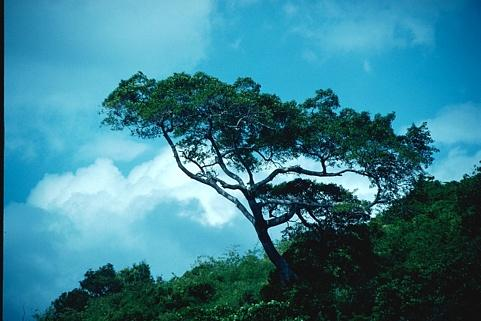
\includegraphics[width=3cm]{images/0.jpg}}
	\subfigure[$k = 2$]
	{
\includegraphics[width=3cm]{images/1.png}}
	\subfigure[$k = 3$]
	{
\includegraphics[width=3cm]{images/2.png}}
	\subfigure[$k = 4$]
	{
\includegraphics[width=3cm]{images/3.png}}
	\caption{Normalized cut usato per la segmentazione di immagini.}
\end{figure}

\section{Insiemi dominanti}

Il concetto di insieme dominante nasce dallo studio sulla formulazione continua del problema della cricca massima su grafi pesati.

Sia dunque $G = (V, E, w)$ un grafo non orientato dove i vertici sono gli oggetti su cui fare clustering, gli archi rappresentano le relazioni tra essi e i pesi rispecchiano la similarità tra coppie di vertici connessi. Sia inoltre $\mat{A} = (a_{ij})$ la matrice di adiacenza pesata.

Si consideri un insieme non vuoto di vertici $S \subseteq V$ e $i \in S$. Il \textbf{grado pesato medio} di $i$ rispetto a $S$ è definito come segue:
\begin{displaymath}
	\textsc{awdeg}_S(i) = \frac{1}{|S|}\sum_{j \in S} a_{ij}
\end{displaymath}
Se $j \notin S$, definiamo
\begin{displaymath}
	\phi_S(i,j) = a_{ij} - \textsc{awdeg}_S(i)
\end{displaymath}
che misura la \textbf{similarità} tra $j$ e $i$ rispetto alla similarità media tra  $i$ e i suoi vicini in $S$.

Il \textbf{peso} di $i$ rispetto ad $S$ è dato dalla definizione ricorsiva
\begin{displaymath}
	w_S(i) = \begin{cases}
		1 & \text{se } |S| = 1 \\
		\displaystyle\sum_{j \in S \setminus \{i\}} \phi_{S \setminus \{i\}} (j, i) w_{S \setminus \{i\}}(j) & \text{altrimenti}
	\end{cases}
\end{displaymath}
ed intuitivamente dà una misura di similarità complessiva tra $i$ e i vertici in $S \setminus \{i\}$ rispetto alla similarità complessiva tra i vertici in $S \setminus \{i\}$.

\noindent Il \textbf{peso totale} di $S$ è:
\begin{displaymath}
	W(S) = \sum_{i \in S} w_S(i)
\end{displaymath}
Vediamo ora come interpretare il significato del peso di un nodo rispetto ad un insieme di vertici. Nel grafo in figura \ref{fig:ds1}, i vertici $\{2,3,4\}$ sono altamente simili tra loro: se proviamo ad aggiungere il vertice $1$, che è dissimile, la similarità complessiva diminuisce, cioè $w_{\{1,2,3,4\}}(1) < 0$. Nel grafo in figura \ref{fig:ds2}, il vertice $5$ è altamente similare ai nodi $\{6,7,8\}$, dunque aggiungendolo all'insieme la similarità complessiva aumenta, cioè $w_{\{5,6,7,8\}}(5) > 0$.

\begin{figure}[h!]
	\centering
	\subfigure[$w_{\{1,2,3,4\}}(1) < 0$]{
	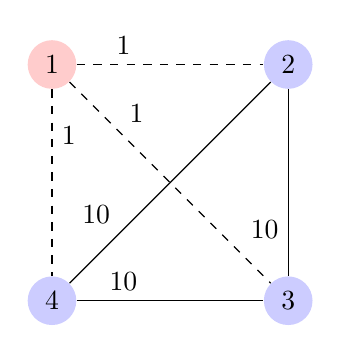
\begin{tikzpicture}[node distance=3cm]
		\node[circle,fill=red!20] (1) at (0,1.5) {1};
		\node[circle,fill=blue!20, right of=1] (2) {2};
		\node[circle,fill=blue!20, below of=1] (4){4};
		\node[circle,fill=blue!20, below of=2] (3) {3};

		\foreach \from / \to in {1/2,1/3,1/4}
		\path (\from) edge[dashed, near start, auto] node{$1$} (\to);

		\foreach \from / \to in {4/2,4/3,3/2}
		\path (\from) edge[near start, auto] node{$10$} (\to);
	\end{tikzpicture}
	\label{fig:ds1}
	}
	\qquad\qquad
	\subfigure[$w_{\{5,6,7,8\}}(5) > 0$]{
	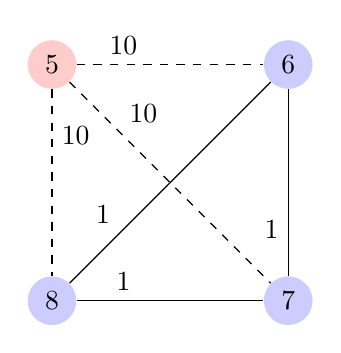
\begin{tikzpicture}[node distance=3cm]
		\node[circle,fill=red!20] (1) at (0,1.5) {5};
		\node[circle,fill=blue!20, right of=1] (2) {6};
		\node[circle,fill=blue!20, below of=1] (4){8};
		\node[circle,fill=blue!20, below of=2] (3) {7};

		\foreach \from / \to in {1/2,1/3,1/4}
		\path (\from) edge[dashed, near start, auto] node{$10$} (\to);

		\foreach \from / \to in {4/2,4/3,3/2}
		\path (\from) edge[near start, auto] node{$1$} (\to);
	\end{tikzpicture}
	\label{fig:ds2}
	}
	\caption[Insiemi dominanti e similarità]{Esempi sui pesi.}
\end{figure}

\noindent È stata dunque definita una misura che descrive cosa comporta, in termini di similarità, l'aggiunta o la rimozione di un nodo. Questo porta alla definizione di insiemi dominanti.
\begin{mydef}[Insieme Dominante]
	Un sottoinsieme di vertici non vuoto $S \subseteq V$ tale che $W(T) > 0$ per ogni insieme non vuoto $T \subseteq S$ è detto \defterm{dominante} se:
	\begin{itemize}
		\item $w_S(i) > 0 \quad \forall i \in S$ (omogeneità interna)
		\item $w_{S \cup \{i\}}(i) < 0 \quad \forall i \notin S$ (disomogeneità esterna)
	\end{itemize}\label{def:domset}
\end{mydef}
\noindent Un insieme dominante è quindi un insieme di vertici massimalmente coesi tra loro e questa definizione corrisponde con quella di cluster.

Quando la matrice di affinità è binaria, l'insieme dominante coincide con la \textbf{clique massimale stretta} in un grafo. Se la disuguaglianza del secondo punto nella definizione \ref{def:domset} non fosse stretta, la clique sarebbe massimale, ma non necessariamente stretta.

\begin{figure}[h!]
	\centering

	\begin{tikzpicture}[node distance=3cm]
		\node[circle,fill=blue!20] (1) at (0,0) {1};
	
		\node[circle,fill=blue!20, below left of=1] (2) {2};
		\node[circle,fill=blue!20, below right of=1] (3) {3};
        
		\node[circle,fill=blue!20, below of=2] (4) {4};
		\node[circle,fill=blue!20, below of=3] (5) {5};

		\foreach \from / \to / \label in {1/2/10,1/3/15,1/4/60,1/5/70}
		\path (\from) edge[near start] node{$\label$} (\to);
		
		\foreach \from / \to / \label in {2/4/25,2/5/20}
		\path (\from) edge[near start] node{$\label$} (\to);

		\foreach \from / \to / \label in {3/4/25,3/5/90}
		\path (\from) edge[near start] node{$\label$} (\to);

		\path (4) edge[auto] node{5} (5);
		\path (2) edge[auto] node{20} (3);

		\begin{pgfonlayer}{background}    % select the background layer
			\fill[gray!20] plot coordinates {(1) (3) (5)};
		\end{pgfonlayer}

	\end{tikzpicture}
	\caption{L'insieme $\{1,3,5\}$ è dominante.}
\end{figure}

\subsection{Gioco del clustering}

Si supponga di avere un insieme di oggetti $O$ ed una matrice di affinità $\mat{A}$, possibilmente asimmetrica, degli elementi di $O$. Due giocatori selezionano contemporaneamente un elemento di $O$ e ricevono un payoff proporzionale all'affinità tra gli oggetti scelti: è dunque nell'interesse di ogni giocatore selezionare un elemento supportato da quelli che l'avversario probabilmente sceglierà.

In questo \textbf{clustering game}:
\begin{itemize}
	\item ci sono due giocatori;
	\item gli oggetti su cui fare clustering sono le strategie pure;
	\item la matrice di affinità (con diagonale nulla) corrisponde alla matrice di similarità.
\end{itemize}

\begin{thm}[A. Torsello, M. Pelillo, S. Rota Bulò, 2006]
	Le strategie evolutivamente stabili nel gioco del clustering con matrice di affinità $\mat{A}$ sono in corrispondenza uno a uno con gli insiemi dominanti.
\end{thm}

\subsection{Insiemi dominanti e affinità simmetriche}

Consideriamo la seguente funzione, che esprime il grado di coesione di un cluster espresso in forma vettoriale $\vec{x}$:
\begin{displaymath}
	f(\vec{x}) = \vec{x}^T \mat{A} \vec{x}
\end{displaymath}
Si può dimostrare il seguente risultato.
\begin{thm}[M. Pavan, M. Pelillo, 2007]
	Se $S$ è un sottoinsieme dominante di vertici, il suo vettore caratteristico $\vec{x}^S$ definito come
	\begin{displaymath}
		x^S_i = \begin{cases}
			\frac{w_S(i)}{W(S)} & \text{se } i \in S \\
			0 & \text{altrimenti}
		\end{cases}
	\end{displaymath}
	è un massimizzatore locale stretto di $f$ in $\Delta$.
	Al contrario, se $\vec{x}^*$ è un massimizzatore locale stretto di $f$ in $\Delta$, il suo supporto $\sigma$ è un insieme dominante, a condizione che $w_{\sigma \cup \{i\}}(i) \neq 0$ per ogni $i \notin \sigma$.
\end{thm}
\noindent La condizione $w_{\sigma \cup \{i\}}(i) \neq 0$ è un tecnicismo dovuto alla presenza di soluzioni spurie. Il teorema può essere visto come la generalizzazione del teorema di Motzkin-Straus ai grafi con archi pesati.

Si può utilizzare una qualunque tecnica di ottimizzazione quadratica per massimizzare $f$ in $\Delta$, tuttavia le \textbf{dinamiche di replicazione} si sono dimostrate lo strumento ideale. Se la matrice di adiacenza $\mat{A}$ è simmetrica, per il teorema della selezione naturale, i punti asintoticamente stabili di una qualunque traiettoria non costante sono in corrispondenza uno a uno con i massimizzatori stretti di $f$ in $\Delta$ e, dunque, con gli insiemi dominanti per la matrice $\mat{A}$.

\subsection{Insiemi dominanti e cluster sovrapposti}

L'idea alla base della tecnica per l'estrazione di cluster possibilmente sovrapposti consiste nel rendere iterativamente \textbf{instabili} le strategie evolutivamente stabili associate agli insiemi dominanti precedentemente estratti: per fare ciò, si introducono \textbf{nuove strategie} nel gioco del clustering che siano best replies solo ed esclusivamente per le ESS già trovate.

Sia $\Sigma$ una tupla di ESS di un gioco con matrice di payoff $\mat{A}$ di dimensione $n \times n$ e sia $\Sigma_i$ l'$i$-esima ESS contenuto nella tupla.

La $\Sigma$-extension $\mat{A}^\Sigma = (a_{ij}^\Sigma)$ della matrice di payoff $\mat{A}$ è definita come
\begin{displaymath}
	a_{ij}^\Sigma = \begin{cases}
		a_{ij} & \text{se } i, j \in \{1, \dots, n\} \\
		\alpha & \text{se } j > n \text{ e } i \notin \sigma(\Sigma_{j - n}) \\
		\beta & \text{se } i, j > n \text{ e } i = j \\
		\frac{1}{|\Sigma_{i - n}|} \sum_{k \in \Sigma_{i - n}} a_{kj} & \text{se } i > n \text{ e } j \in \sigma(\Sigma_{i - n}) \\
		0 & \text{altrimenti}
	\end{cases}
\end{displaymath}
dove $\alpha > \beta$ e $\beta = \max_{i, j} a_{ij}$.

\begin{thm}[A. Torsello, M. Pelillo, S. Rota Bulò, 2008]
	Sia $\Phi$ un gioco doppiamente simmetrico a due giocatori con matrice di payoff $\mat{A}$ e sia $\Sigma$ una tupla di ESS di $\Phi$. Sia inoltre $\Phi^\Sigma$ un gioco a due giocatori con matrice di payoff $\mat{A}^\Sigma$. Allora $\vec{x}$ è una ESS di $\Phi$ non in $\Sigma$ se e solo se $\vec{x}$ è una ESS di $\Phi^\Sigma$.
\end{thm}

\noindent Un esempio di $\Sigma$-extension segue.

\begin{minipage}[c]{0.49\textwidth}
	\begin{center}
		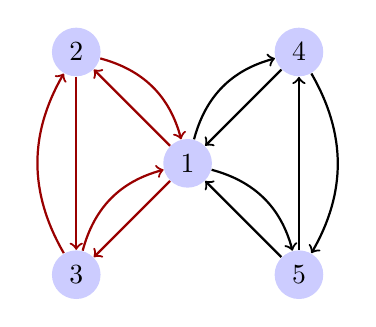
\begin{tikzpicture}[->, node distance=2cm]
			\node[circle, fill=blue!20] (1) at (0,0) {1};
		
			\node[circle, fill=blue!20, above left of=1] (2) {2};
			\node[circle, fill=blue!20, below left of=1] (3) {3};
	        
			\node[circle, fill=blue!20, above right of=1] (4) {4};
			\node[circle, fill=blue!20, below right of=1] (5) {5};
	
			\foreach \from / \to in {1/2,1/3,2/3} {
				\path (\from) edge[thick, near start, color=black!40!red] (\to);
				\path (\to) edge[bend left, thick, near start, color=black!40!red] (\from);
			}
			
			\foreach \from / \to in {1/4,1/5,4/5} {
				\path (\from) edge[bend left, thick, near start] (\to);
				\path (\to) edge[thick, near start] (\from);
			}
		\end{tikzpicture}
	\end{center}
\end{minipage}
\begin{minipage}[c]{0.49\textwidth}
	\begin{center}
		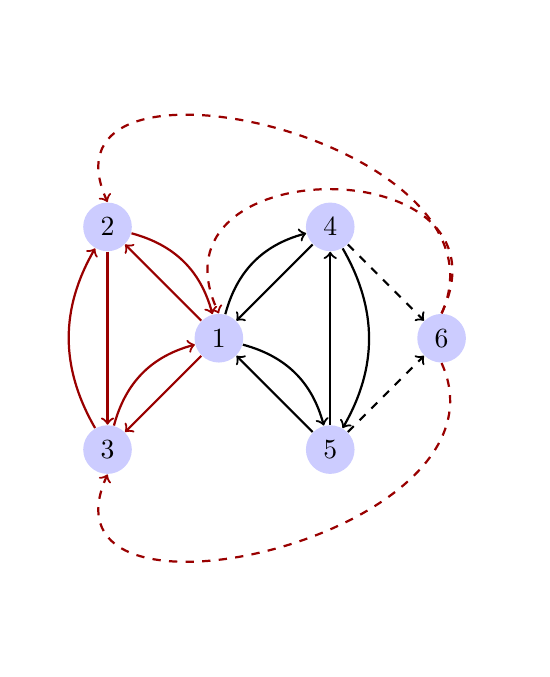
\begin{tikzpicture}[->, node distance=2cm]
			\node[circle,fill=blue!20] (1) at (0,0) {1};
		
			\node[circle, fill=blue!20, above left of=1] (2) {2};
			\node[circle, fill=blue!20, below left of=1] (3) {3};
	        
			\node[circle, fill=blue!20, above right of=1] (4) {4};
			\node[circle, fill=blue!20, below right of=1] (5) {5};
			
			\node[circle, fill=blue!20, below right of=4] (6) {6};
	
			\foreach \from / \to in {1/2,1/3,2/3} {
				\path (\from) edge[thick, near start, color=black!40!red] (\to);
				\path (\to) edge[bend left, thick, near start, color=black!40!red] (\from);
			}
			
			\foreach \from / \to in {1/4,1/5,4/5} {
				\path (\from) edge[bend left, thick, near start] (\to);
				\path (\to) edge[thick, near start] (\from);
			}
			
			\foreach \from / \to in {4/6,5/6}
				\path (\from) edge[thick, dashed, near start] (\to);
			
			\draw [->, color=black!40!red, thick, dashed] (6.north) .. controls +(1,2.1) and +(-1,2.1) .. (1.north);
			\draw [->, color=black!40!red, thick, dashed] (6.north) .. controls +(1,2.2) and +(-1,2.2) .. (2.north);
			\draw [->, color=black!40!red, thick, dashed] (6.south) .. controls +(1,-2.2) and +(-1,-2.2) .. (3.south);			
		\end{tikzpicture}
	\end{center}
\end{minipage}

\noindent Supponiamo che l'insieme dominante $D = \{1, 2, 3\}$ sia stato estratto e non si voglia più ottenerlo in futuro: per fare ciò si introduce un nuovo nodo ($6$), si crea un arco $(n, 6)$ per ogni $n \notin D$ e un arco $(6, n)$ per ogni $n \in D$. I pesi sono impostati in accordo alla formula data sopra.

\subsection{Insiemi dominanti e partizionamento}

Anche se gli insiemi dominanti sono stati introdotti con il preciso scopo di superare l'approccio classico al clustering, visto come un problema di partizionamento, è comunque possibile creare una partizione dei dati in ingresso, secondo la strategia \textbf{peel-off}. L'algoritmo è il seguente:
\begin{algorithmic}[1]
	\State Trova un insieme dominante.
	\State Rimuovilo dal grafo.
	\State Torna al punto 1 se il grafo contiene ancora dei vertici.
\end{algorithmic}
Il problema di questo approccio è dovuto al fatto che la rimozione di vertici introduce un \textbf{implicito cambio di scala} per quanto riguarda i pesi degli archi.